\section{The Great Loop Trip}

\margininbox{Vrtnarija round trip}{
     \begin{itemize}
    \item Jarvist Frost
    \item Dan Greenwald
    \end{itemize}}{\explo}

Dan and I are men that like missions. This is a polite way of saying
that in our laziness, we suddenly arrive at the last minute and find
that the only way to achieve the bare minimum of what we planned, is to
pull an all nighter. Or several.

And so we had a plan. A photograph, camp, push, survey, derig plan. We
zoomed down the main pitch series in \passage{Vrtnarija} with a tackle sac
each. I hadn't been below \passage{Pico} since 2004, Dan had never gone
past the \passage{Captain Kangaroo} window. I led with the camera, Dan
followed with the flash unit. It was an interesting experience
remembering the pitch series that I had glimpsed just once, five years
previously. \bignote{The rope was old, so very old}. I made the mistake of looking
for the label on \passage{Concorde} while waiting for Dan to catch up.
`ICCC - 1998 - 90 m'. Nice, old club rope that had been `disposed' of by
hiding underground in Slovenia.


\begin{pagefigure}
\checkoddpage \ifoddpage \forcerectofloat \else \forceversofloat \fi
\centering
 \frame{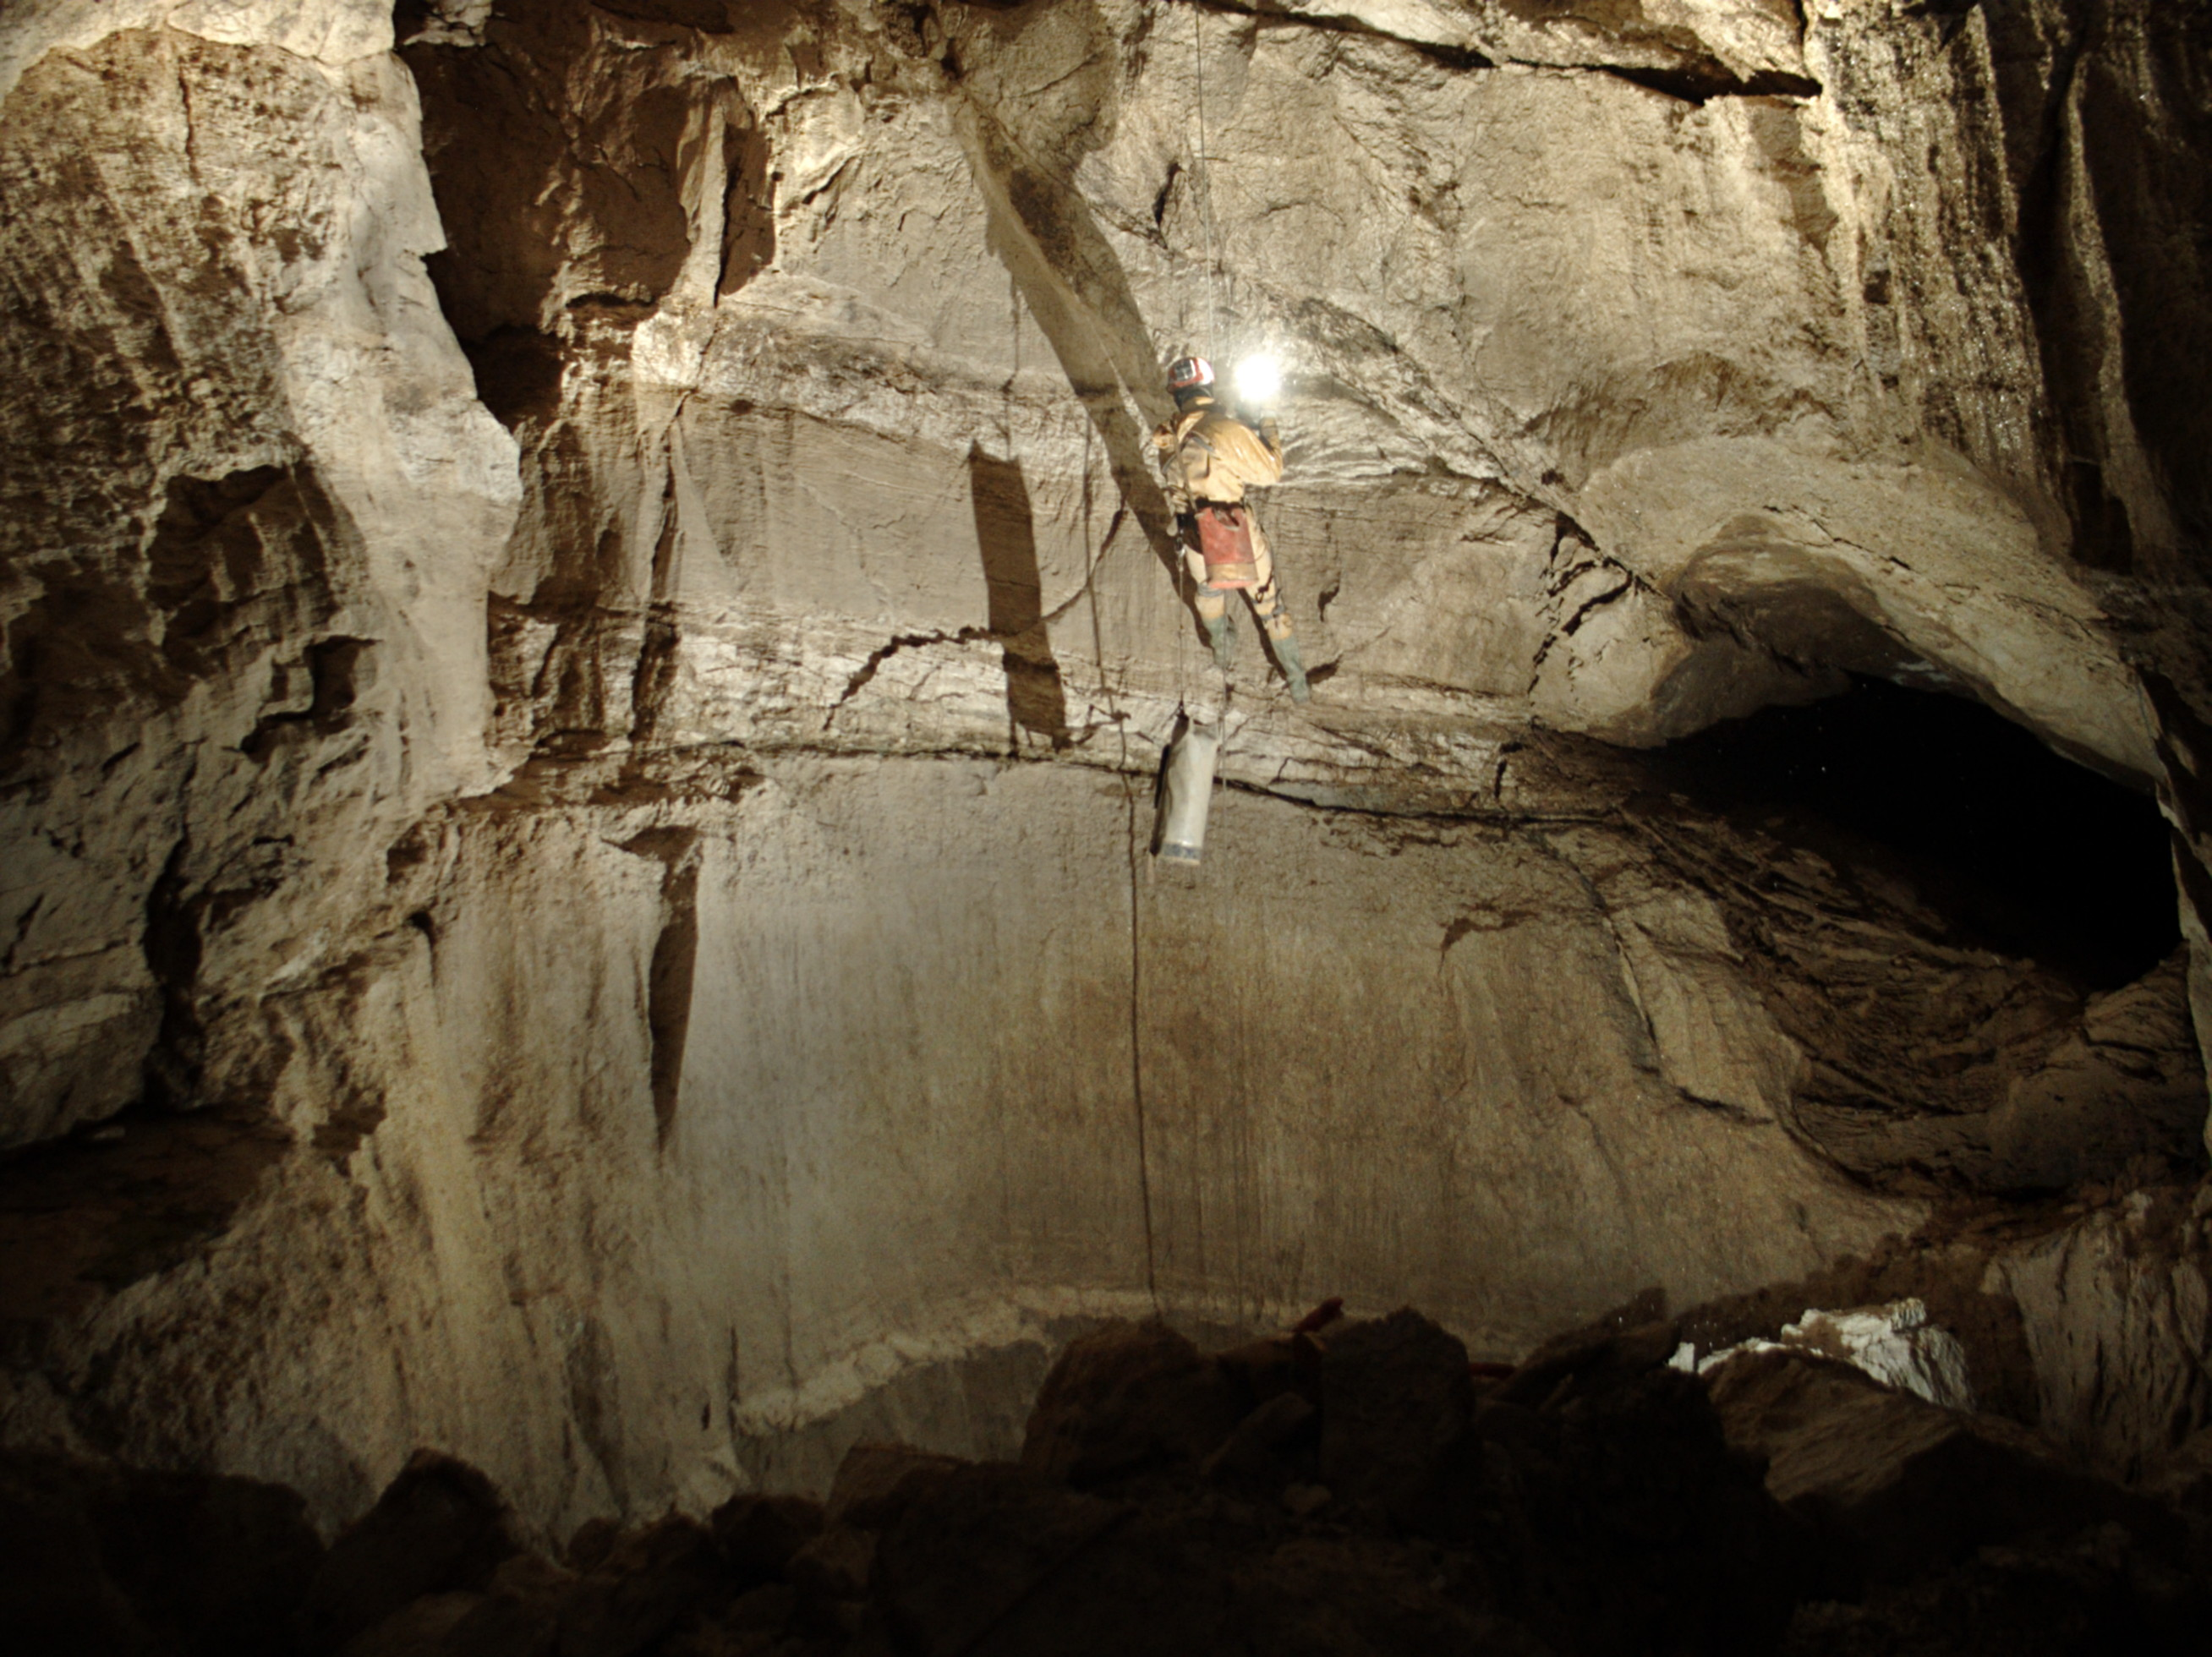
\includegraphics[width=\textwidth]{2009/great_loop/2009-08-16-14.52.26 - Jarvist Frost - Canon Powershot G5 - zimmer bottom of pitch with friendship and leopard--orig.jpg}} 
 \caption{Dan abseiling to the bottom of \protect\passage{Zimmer}. The window to \protect\passage{Leopard} is visible to his upper left; the entrance to \protect\passage{Friendship Gallery} is on the right. \pic{Jarvist Frost}}
 \label{leopard friendship}
\end{pagefigure}


In all honesty, it was all a bit of a mess. Piecemeal upgrades had taken
place in 2007 and 2008, but already the `new' rope was looking
increasingly indistinguishable from the stuff that had been in situ
since 2003. And of course, being us, we had no records of exactly what
had been replaced.

It was quite a relief to get off at the foot of \passage{Zimmer} (the
shrunken rope and badly located original rebelay required some rather
innovative gymnastics). \passage{Zimmer} itself was an extremely impressive
place for the first time visitor - it's a big chamber, and by far the
larger volume of water comes in from the far side of the shaft. Where
does the water come from? Nobody knows.

Seeing it for the first time, the simple existence of \passage{Leopard} was
amazing, you could see the same band of rock extending across the
\passage{Zimmer} shaft from the (free climbable) window into \passage{Friendship Gallery}. There was clearly excellent potential.

Similarly, we followed the obvious gaping corridor down \passage{Tolminska
Korita}\sidenote{Though the \passage{Tolminska Korita} survey data follows \passage{Below Zimmer} and relates to cave passage pushed in 2010, this area was always known as \passage{Korita}}. This was in fact the obvious way on from the \passage{Zimmer}
chamber, quickly collecting the pitch water that flowed down between the
boulders. Only two pitches were rigged, but they were really quite
beautiful. Y-hangs in a narrow rift popped out into perfect bell-jar
hangs next to picturesque splash pools. Such an amazing lead to push
next year.

\begingroup
\setlength{\fboxrule}{0pt}
\begin{figure*}[t!]
\checkoddpage \ifoddpage \forcerectofloat \else \forceversofloat \fi
\centering
 \frame{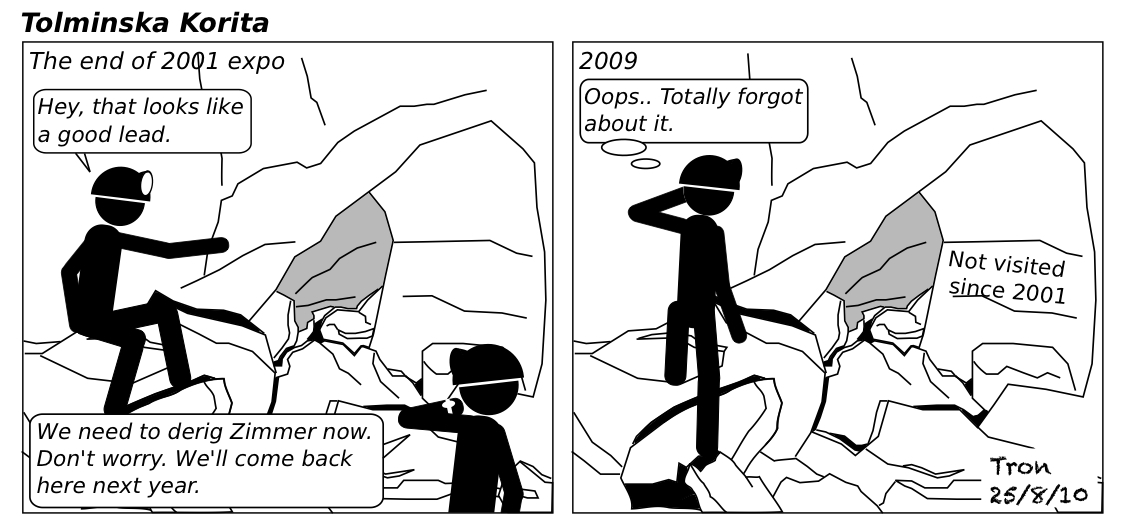
\includegraphics[width=\textwidth]{2009/great_loop/Tharatorn Supasiti - March 2012 - korita--orig.jpg}} 
 \caption{An impression of forgotten leads. \pen{Tharatorn Supasiti}}
 \label{korita ignored}
\end{figure*}
\endgroup



Our photographs taken, we returned to \passage{Zimmer} pulling up the
ropes. James and Tim were planning to return on a bounce trip here to
push the next pitch\sidenote{\protect\passage{Eggsplosive}, see overleaf}. Dan \& I started down \passage{Friendship Gallery} -
impressive for its horizontal nature in such an aggressively vertical
system, but otherwise a rather muddy place. Camp \passage{X-Ray} was made
obvious by the inevitable presence of a roll of dubious plastic bags,
and a rusty tin of fish. It was not the most pretty of oxbows, but the
floor was fairly flat and the plinth of dry-stone walling was obviously
big enough for a 4-man tent.


\begin{figure}
\checkoddpage \ifoddpage \forcerectofloat \else \forceversofloat \fi
\centering
 \frame{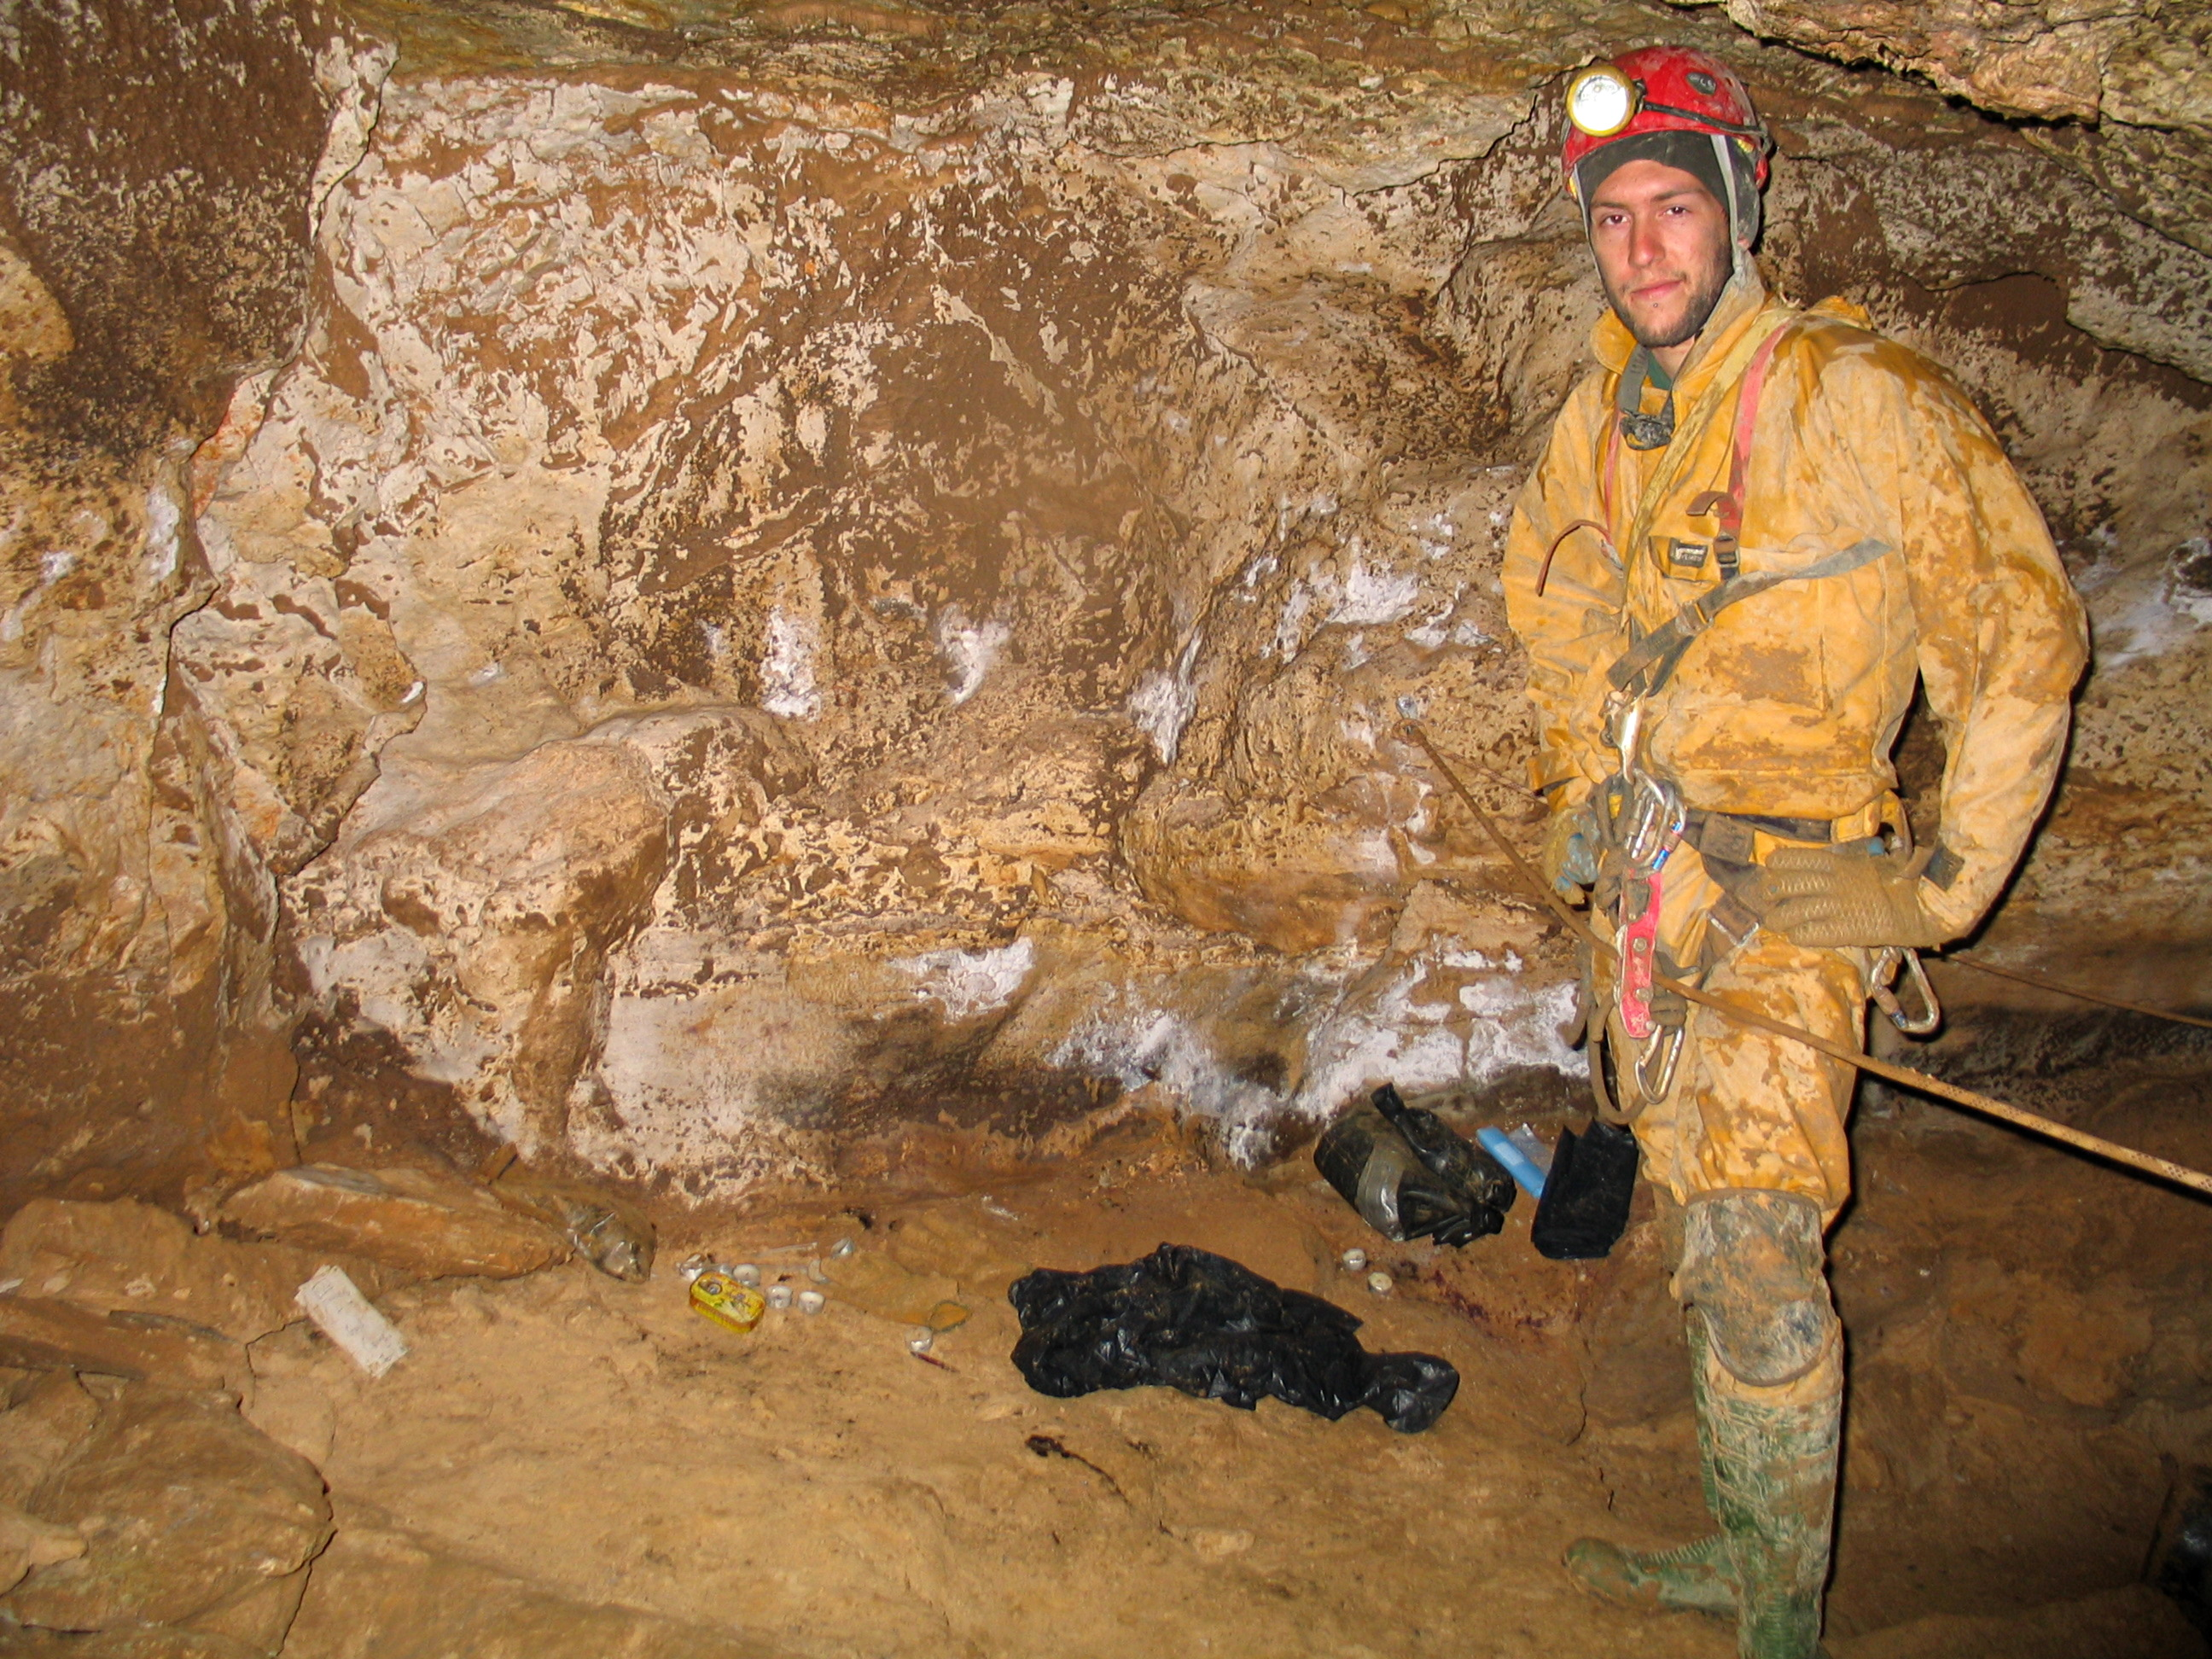
\includegraphics[width=\linewidth]{2009/great_loop/2009-08-16-15.47.29 - Jarvist Frost - Canon Powershot G5 - Camp X-ray visit--orig.jpg}} 
 \caption{Dan at \protect\passage{Camp X-Ray}, 6 years after it was last used for underground camping. \pic{Jarvist Frost}}
 \label{xray 2009}
\end{figure}




    \margininbox{Eggsplosive}{
     \begin{itemize}
    \item James Kirkpatrick
    \item Tim Osborne
    \end{itemize}}{\explo}


Directly after the site of the camp, there were some rather rubbish
roped climbs. The muddy rock had been turned into slippery slopes by the
passage of many cavers, but beyond the climbs was a beautiful crawlway
half filled with a perfectly flat layer of silt. The crawl turned into a
stoop and then a run down a slope to the obvious \passage{Prima Junction}.

Our aim here was to tie in the survey. Finding the PSS at \passage{Prima
Junction} was a joke. We had read the description, but the cairn must
have been kicked away many years ago. A few minutes were spent rifling
through the boulders in case the PSS paper had escaped, but it was a
dead loss.


\begin{marginfigure}
\checkoddpage \ifoddpage \forcerectofloat \else \forceversofloat \fi
\centering
 \frame{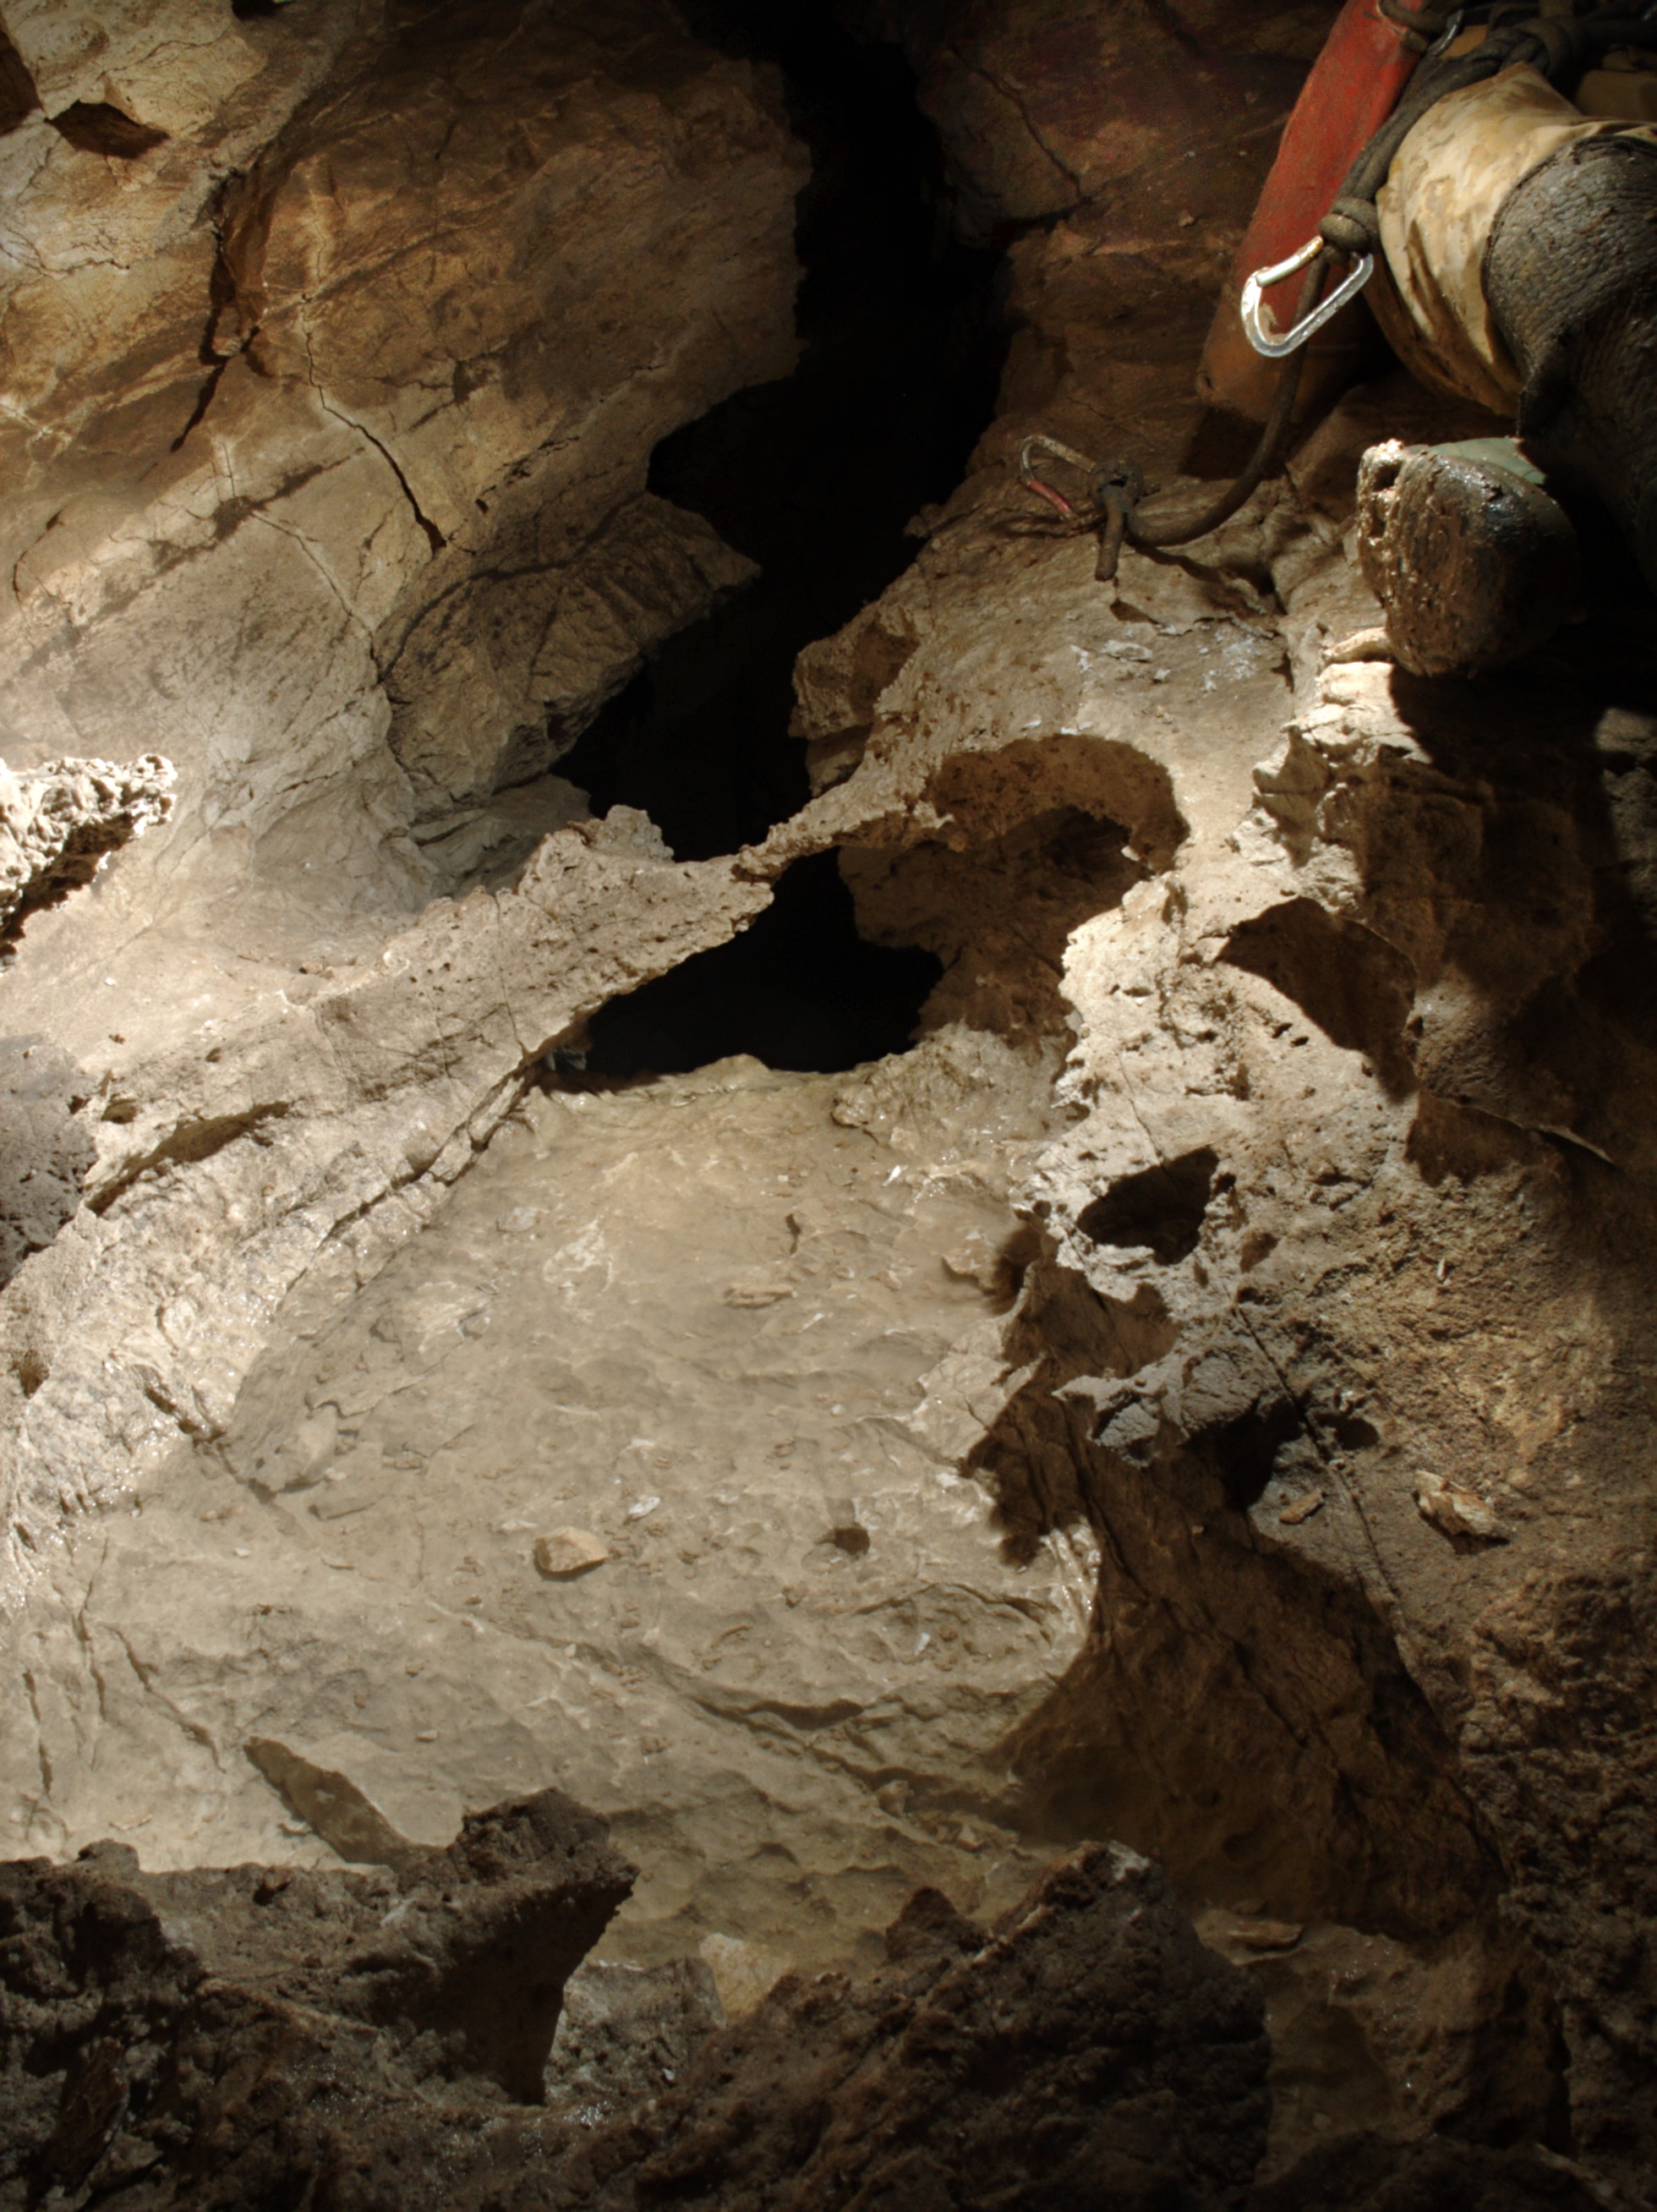
\includegraphics[width=\linewidth]{2009/zimmer/2009-08-16-15.13.32 - Jarvist Frost - Canon Powershot G5 - Eggstacy - below zimmer - rock bridge at head of unpushed 2nd pitch--orig.jpg}} 
 \caption{The head of \protect\passage{Eggsplosive} pitch, pushed by James and Tim and left as a going lead for 2010. \pic{Jarvist Frost}}
 \label{below zimmer second pitch eggsplosive}
\end{marginfigure}


So we guessed where we'd put the PSS, and threaded a survey down through
the boulders, finding the rope that Dave had rigged. The rusty old bolt
on the ledge was an obvious place to put a survey station in, but we
also bounced down to the start of the \passage{Falls Road}. Tim's crazed
traverse on sling hung naturals took you across to the other side of
this confluence, a smaller stream that quite possibly leads from
underneath \passage{Friendship Gallery}. And the way down looked pretty
exciting too. We had been told that it ends at a narrowing, but
certainly the start of the pitches were something that after having
forced \passage{Captain Kangaroo} to a successful conclusion would not turn
us away.

Most strange of all, the way back into the bottom of \passage{Captain
Kangaroo}, \passage{Free Amalgamation} was an obvious crawlway leading off
from exactly where the \passage{Falls road} explorers had stopped to bolt.
I can only assume they were so obsessed with heading down that they
never stopped to turn around and look at the massive rift disappearing
off.

Dan and I zoomed along this beautiful bit of cave, soon coming out into
a clambering rift that leads to the \passage{Hanging Garden}. Why they
didn't come here in 2003 I will never understand. This was a rather
distressing place to be. Three large blocks dangled from the ceiling.
You could see that the largest was held up by the bedrock on the walls,
but you could also see how this had been pulverised into shattered
pebbles and the boulder slid into place. The thin rope led off up into
the ceiling.


\begin{marginfigure}
\checkoddpage \ifoddpage \forcerectofloat \else \forceversofloat \fi
\centering
 \frame{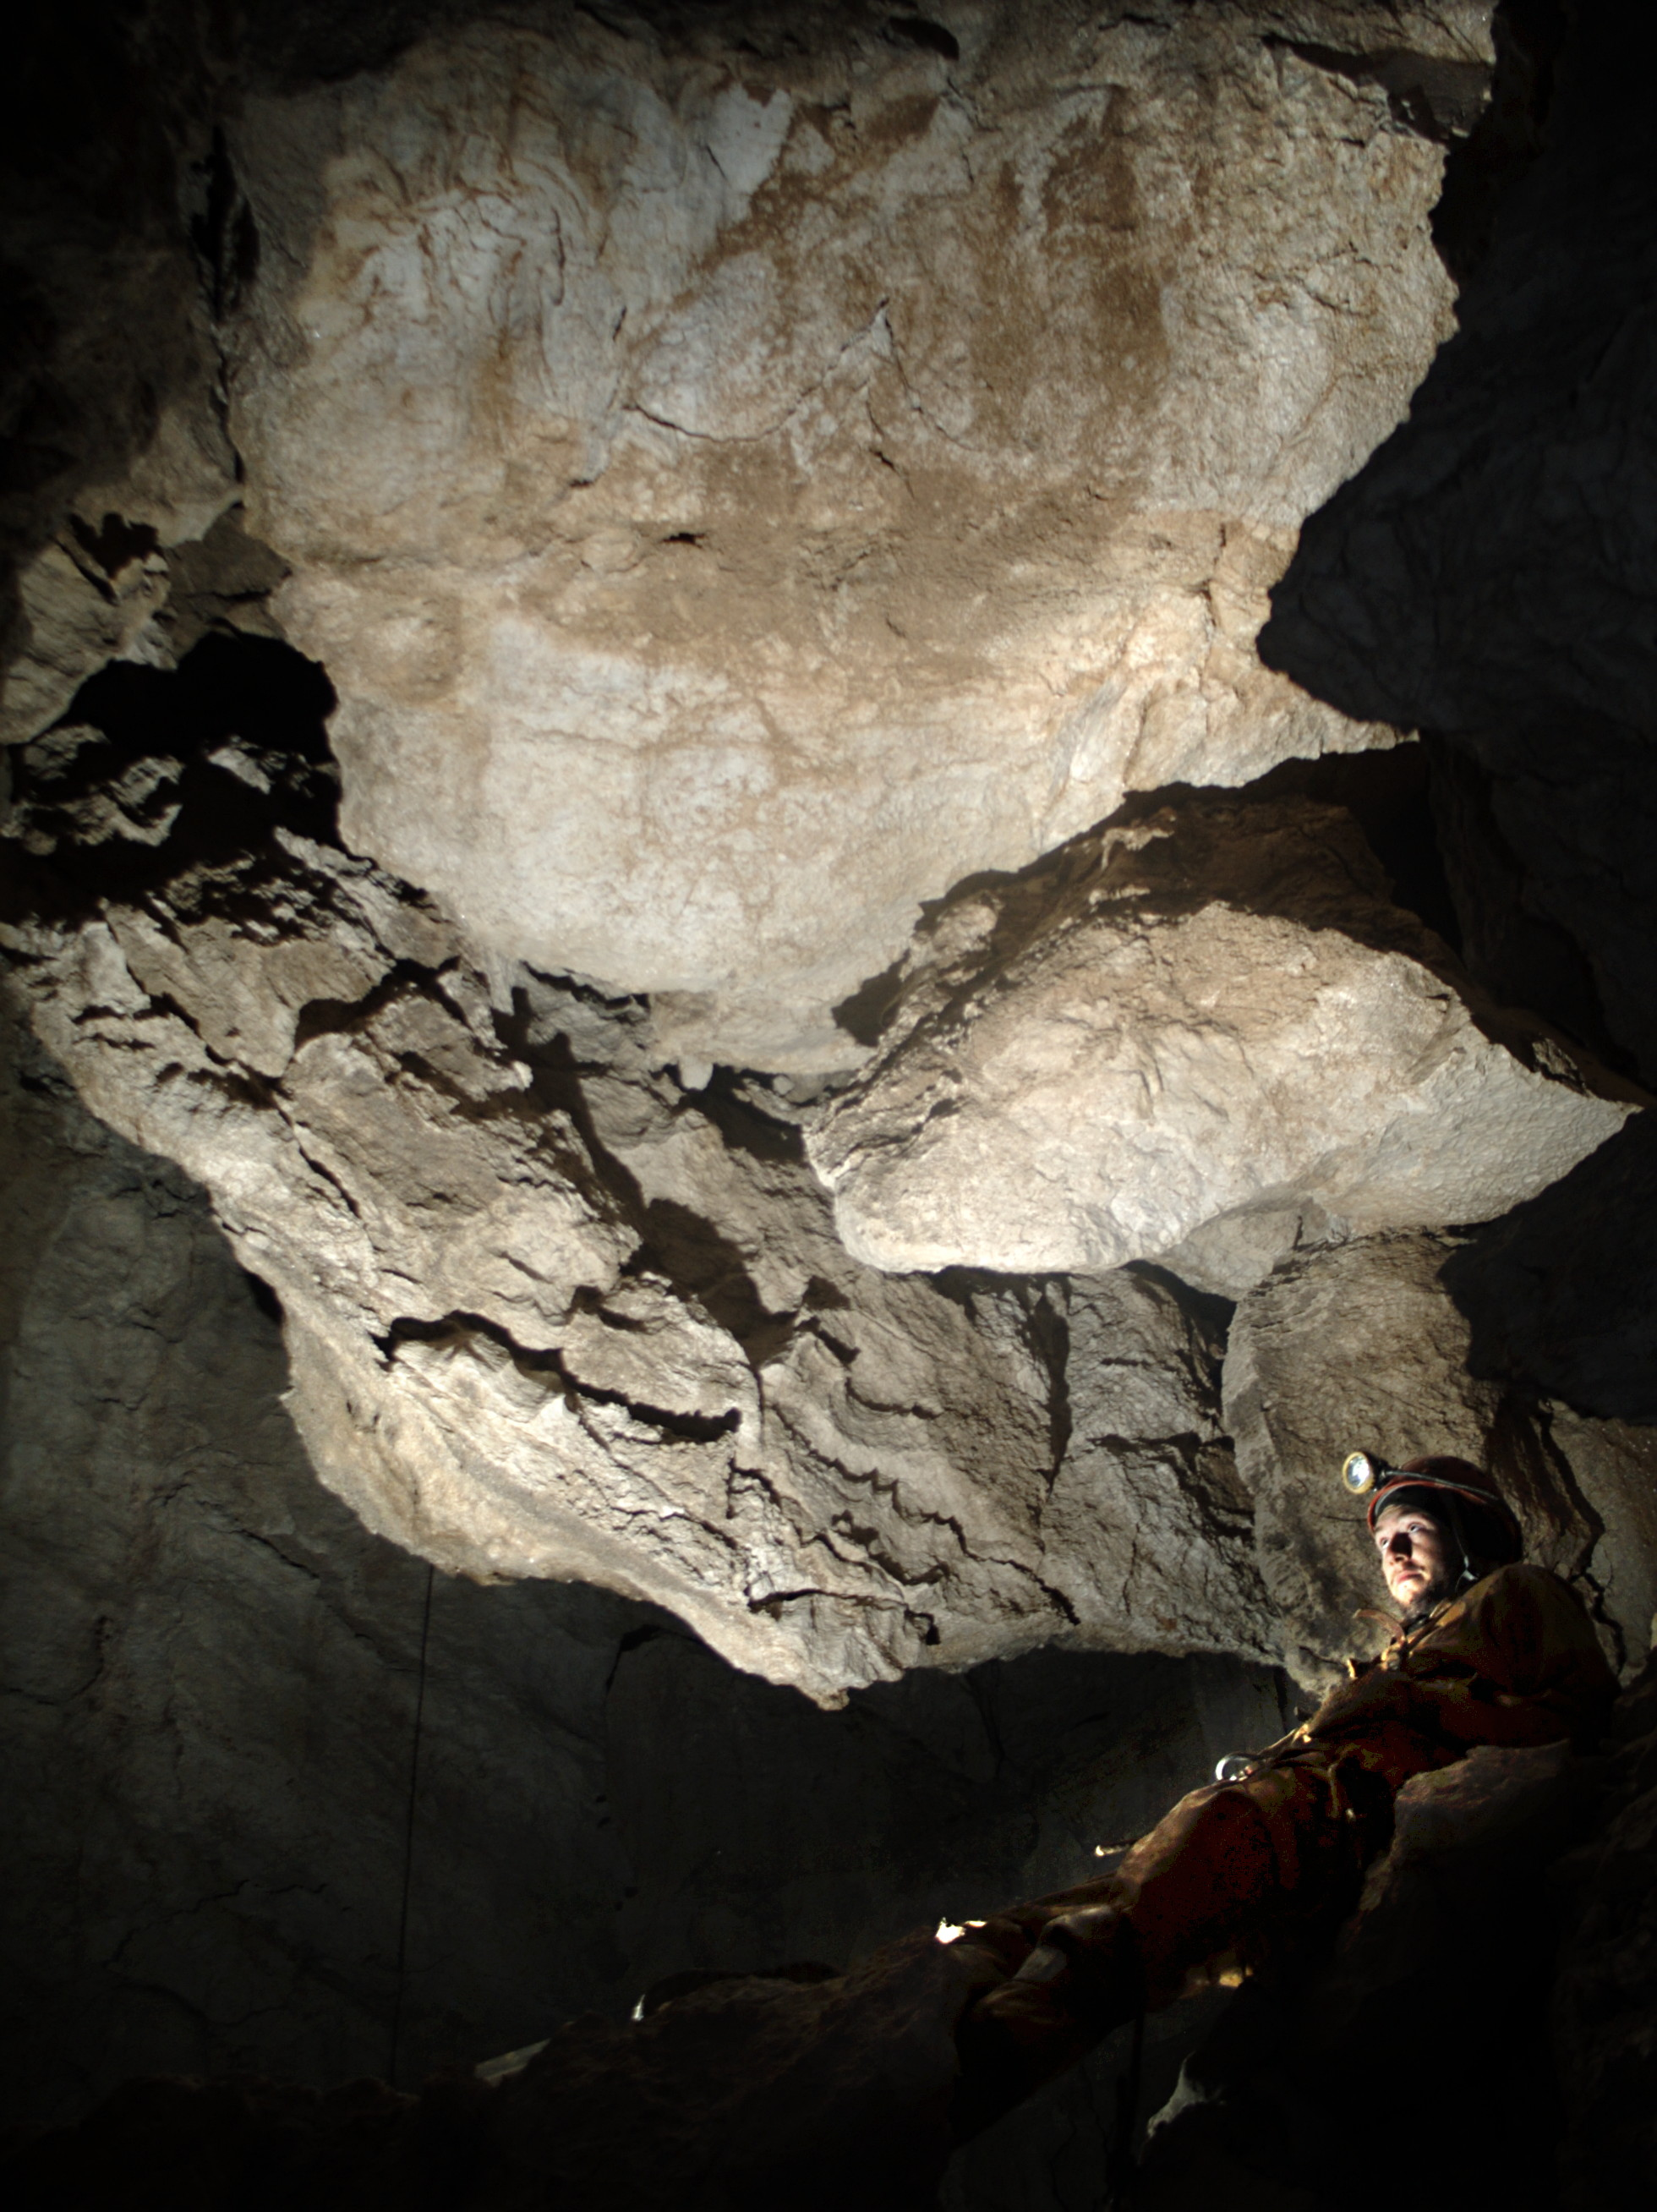
\includegraphics[width=\linewidth]{2009/great_loop/2009-08-16-16.42.38 - Jarvist Frost - hanging garden - dan looking rather worried--orig.jpg}} 
 \caption{Dan beneath the hanging death. \pic{Jarvist Frost}}
 \label{Hanging Garden}
\end{marginfigure}

Following this, taking care to flick the rope away from the tiny stream
and so keep it serviceable for people entering next year from below, a
tiny bit of boulder choke finds you at the bottom of the impressive
\passage{Happy Monday}.


\begin{pagefigure}
\checkoddpage \ifoddpage \forcerectofloat \else \forceversofloat \fi
\centering
 \frame{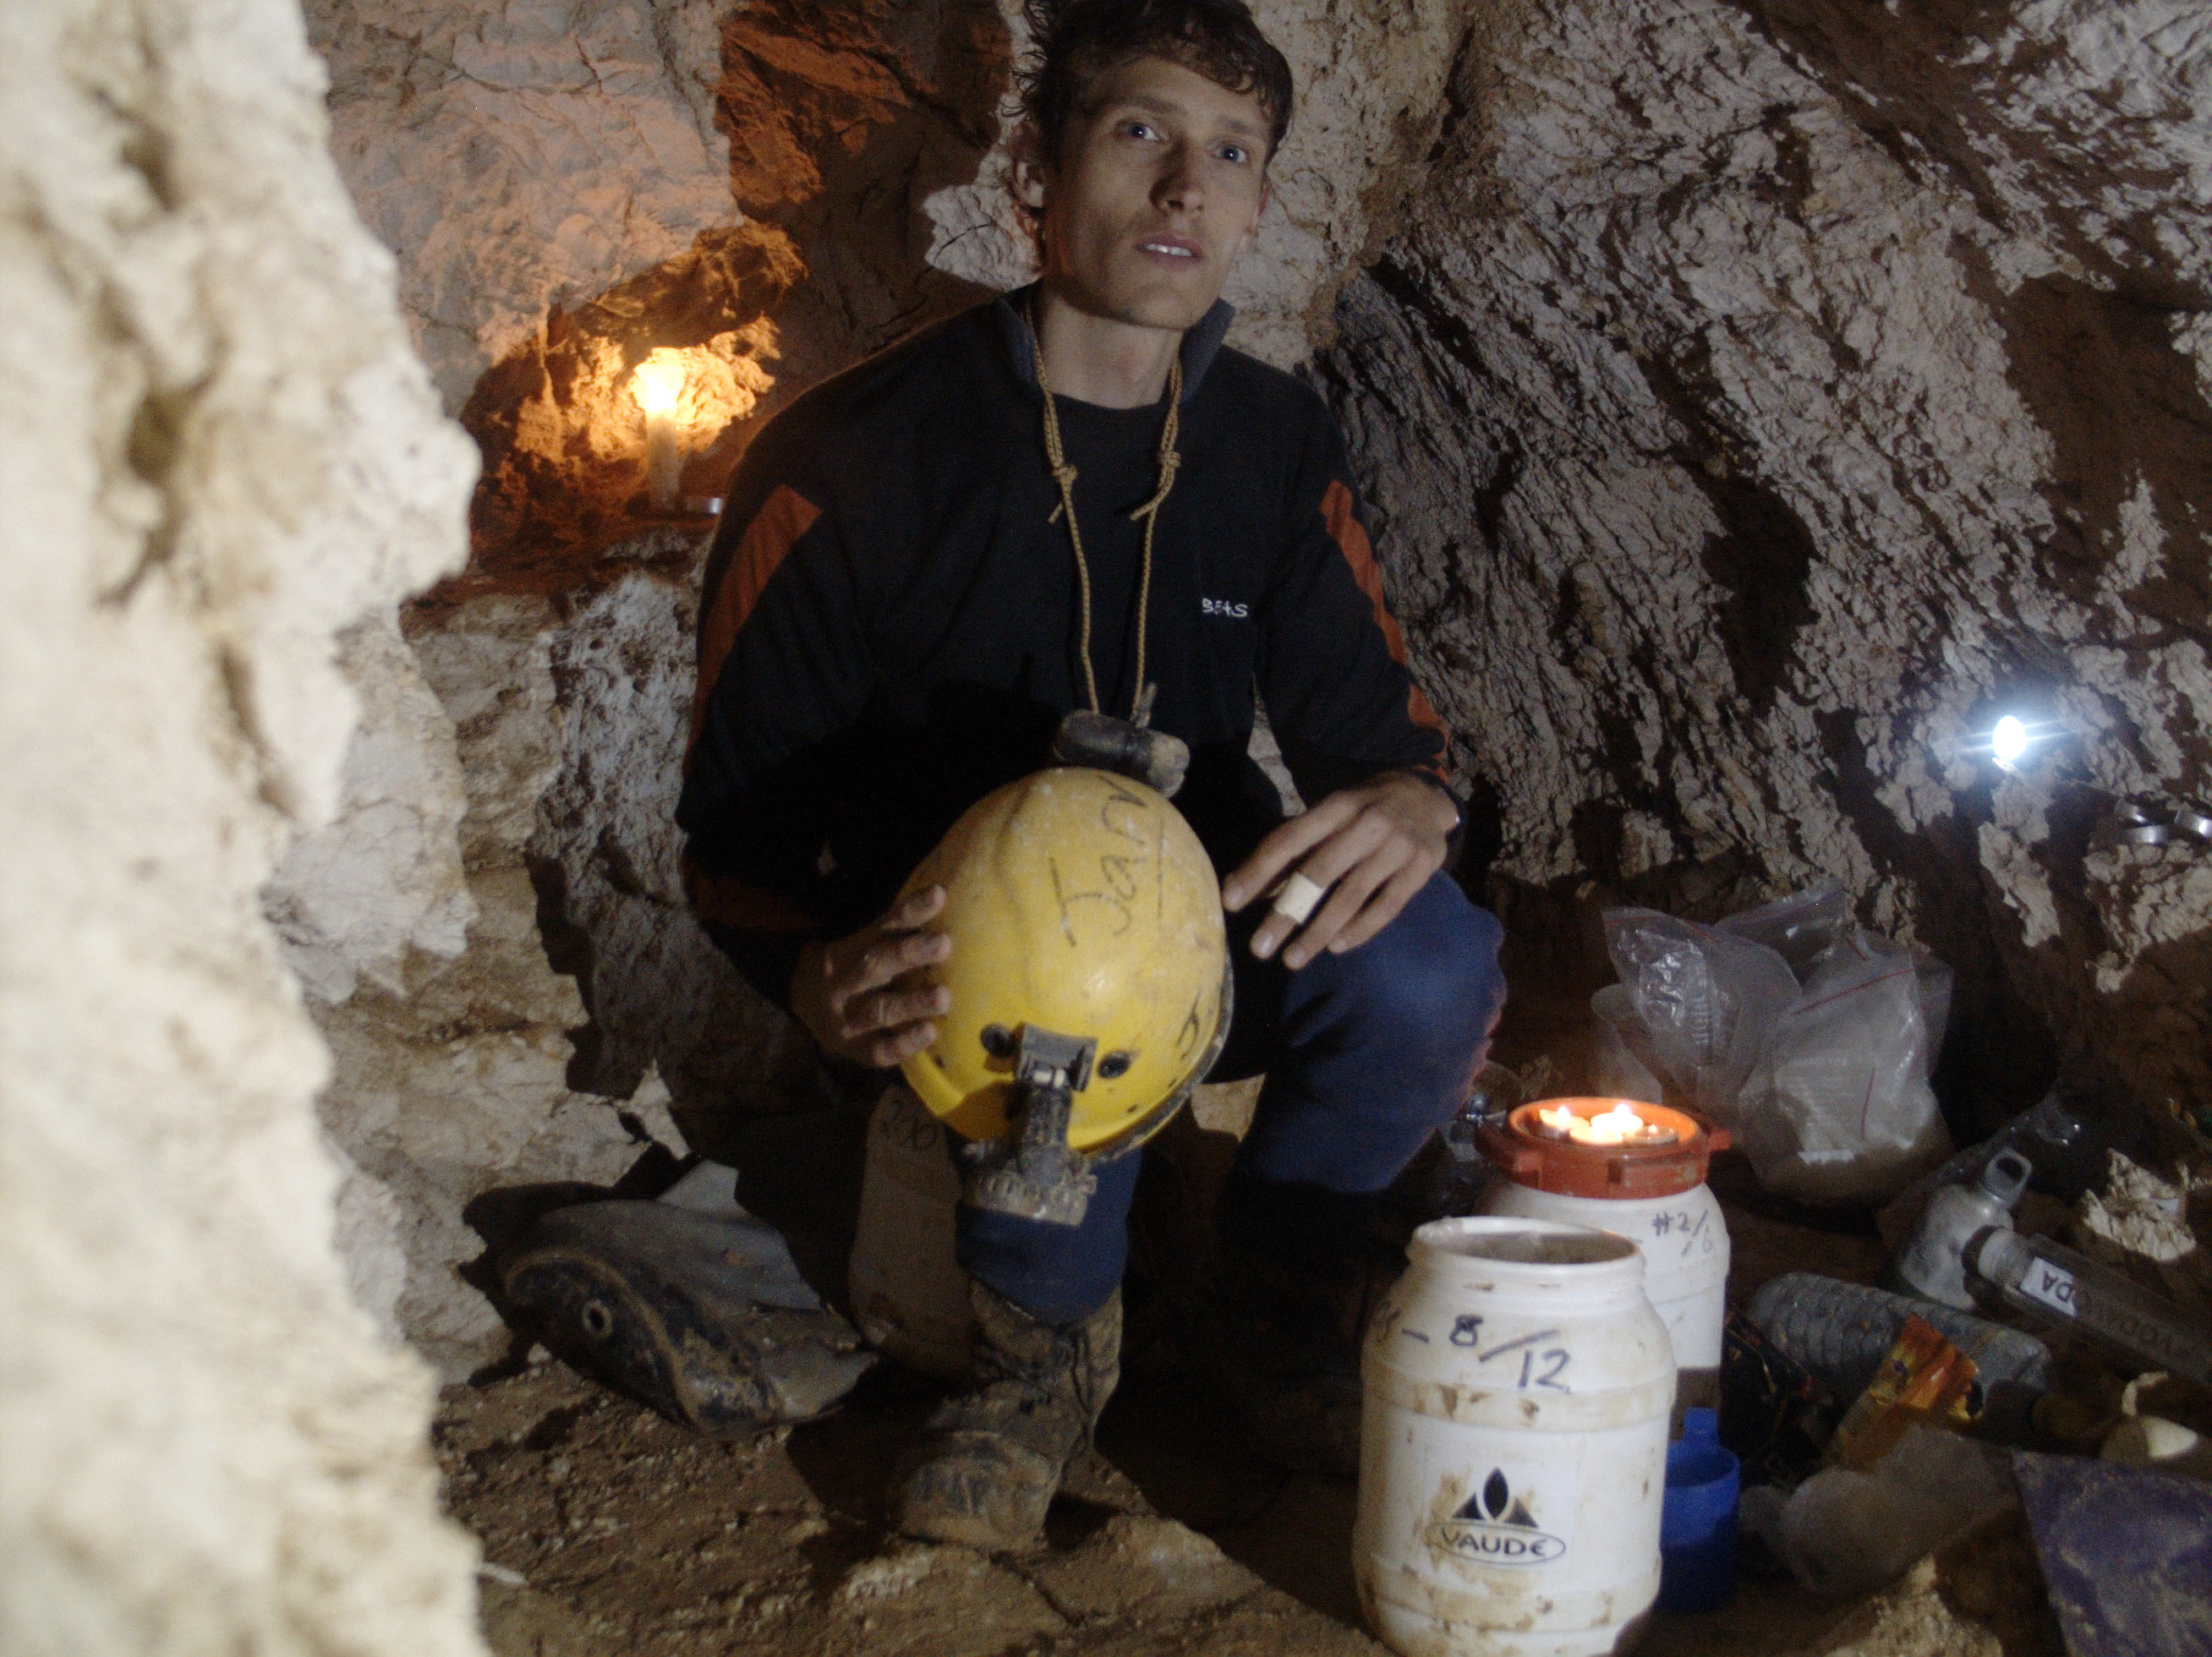
\includegraphics[width=\textwidth]{2009/great_loop/2009-08-05-21.22.06 - Jarvist Frost - Canon Powershot G5 - Jarv in camp by LED light--orig.jpg}} 
 \caption{The 2009 expedition was sponsored by BEAST, who donated sets of thermals that helped make underground camping comfortable. \pic{Mike Foley}}
 \label{beast thermals}
\end{pagefigure}

\tweet{1:24PM Aug 19th, 2009}{Caves derigged! Last camp a bit of an epic photo, survey, push, via zimmer and then up into metal camp. Carries today, last bit of surve ...}

What a pitch! It's truly massive. We measured it with the tape - a true
twenty by twenty metres. We added PSS Zero on the obelisk like boulder
in the centre of the chamber (the original PSS at the bottom of the thin
9 mm disappearing into the ceiling was getting repeatedly kicked over).
The walls just went up and up, a massive Toblerone prism extending up
into the blackness. Skidding around on the scree to get a good position
to photograph Dan. The 9 mm rope rising from the middle of this chamber
and disappearing into blackness is simultaneously foreboding and alien.

The \passage{Muddy Window} is enticing indeed, but how to reach it, a good
ten metres off the ground? The length of the lower hang is so great that
we reckon we can swing\ldots{} Halfway up and \bignote{with Dan pulling the rope
tail in synchronisation, I fly backwards and forwards pinwheeling my
legs} to retain attitude. Dan stumbles and nearly breaks a leg granting
me my delta-V. I fly in and nearly kiss the rock, abseil down another
metre and with a final pull from Dan and then the terrifying build of
rushing wind as I accelerate towards my destiny, I enter the window and
abseil to the ground, landing in a boulder filled corridor.

I shout an OK to Dan and pull up the rope behind me, wrapping it around a
few blocks. The corridor leads through a stoop and then to a chamber
filled with heavy chocolate mud covered boulders. There is an extremely
noticeable draught here. The mud is extremely odd, it's not obvious how
it could have been carried by water. Earthquake driven liquefaction is
Dan's best guess. The way on is obvious - from this chamber there's an
easy climb up and to the right gaining a horizontal continuation.

I return to Dan, and have the bolting kit passed up. I start to put in a
bolt but it's a challenging position and time is marching on. We give up
and leave it for next year. Dan is swung into the window to have a look,
and then we make haste for \passage{Metal Camp}, after the necessary photo.


\recipecorner{Metal Camp menu}{
\begin{itemize}
    \item Couscous, smash, fish and smash with tomatoes 
    \item Smash, smash, smash, cheese and fish
    \item Couscous, fish, tomato, couscous and cheese.
\end{itemize}
\mininame{Thara}}


Dan prussics up with the camera flash, I blow my whistle when I think he
should fire a flash. As well as the film camera balanced on the obelisk
rock I'm lying flat on my back on the scree with my digital camera,
trying to synchronise a long exposure with when he's firing the
individual flashes flash. So peaceful to watch from below, the entire
pitch seared with persistence of vision onto my retina. As he passes the
rebelay, Dan disappears behind a flake that divides the top of the shaft
into two bits (damn! not that there would have been anyway to predict
this from below\ldots{}). But still the flash illuminates from behind
this flake, a truly enormous and humbling place to be.

Dan successfully up, I shake the sluggish blood from my extremities and
shiver as I pack up the photo gear and prepare to climb.

The pitch itself passes without incident, but 81 m seems a little long
to do with a single rebelay! The 10 m horizontal swing onto `Spelenium
Gold' dyneema rope at the rebelay is a little bit too life affirming.

The trudge back to camp is rather soul sapping. I curse my camera
equipment as I wrestle it, once more, through \passage{Kill'em All}. Sad
times at camp to think that our little hovel, our little bolthole in the
side of a pitch cascade, will soon be abandoned. Having made the
connection and seen the pleasant environment at \passage{X-Ray}, I doubt
very much that this strange little side chamber will ever be occupied
again.

\margininbox{Camp in hindsight}{In retrospective the most memorable things [about 2009] were how cosy the campsite seemed, but how horrid it was, pissing in a box etc etc etc. and how it would constantly crumble rocks on top of it. \mininame{James Kirkpatrick, 2011}}{\logbook}

Dan smokes a last cigarette before sleep, the Jonny Cash playing softly
on the radio.

The next day, stiff and tired, we head down once again. Our mission is
to survey, then derig. The photo gear is left at camp, but still the
trip feels rather arduous and not very rewarding.

The rope is pulled up all the pitches, and coiled somewhere suitable.
Another quiet evening in camp and some needed rest.


\begin{figure}
\checkoddpage \ifoddpage \forcerectofloat \else \forceversofloat \fi
\centering
 \frame{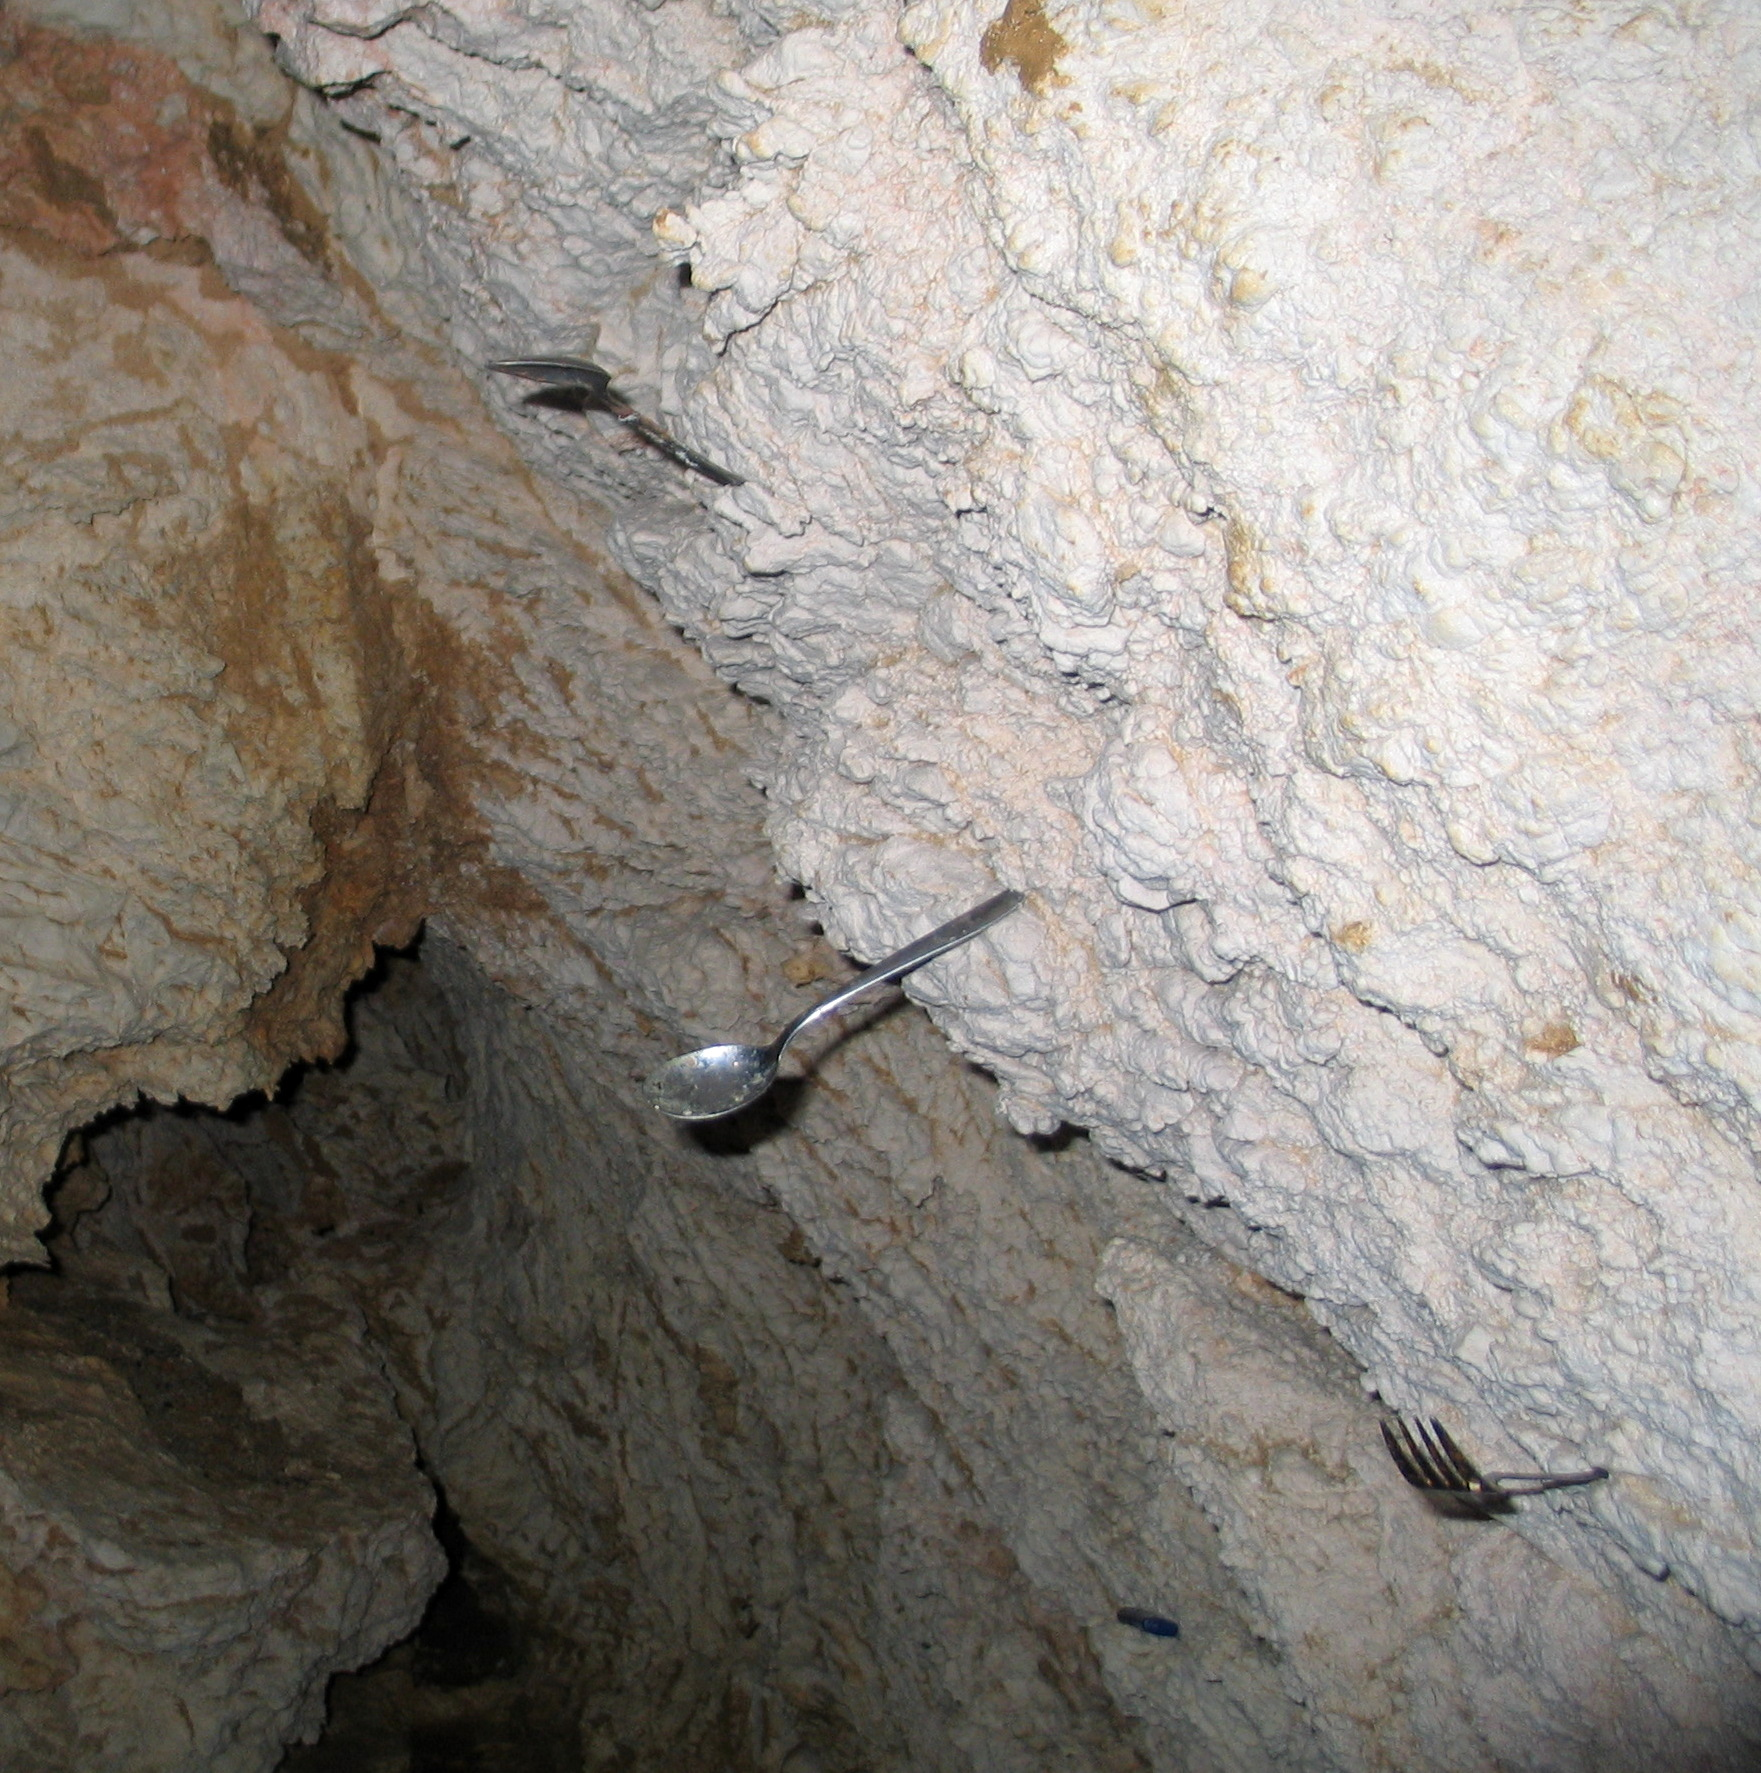
\includegraphics[width=\linewidth]{2009/great_loop/2009-08-18-10.31.26 - Jarvist Frost - Canon Powershot G5 - Last Camp - spoon garden2--orig.jpg}} 
 \caption{The spoon garden. \pic{Jarvist Frost}}
 \label{spoons}
\end{figure}


\margininbox{Herman Herz, 2010}{
     "Grigory Perelman (nom de plume, AKA William French) - for everything from freeclimbing to the bottom of \protect\passage{S1} (having passed the pitch rigger on the way down somehow), getting down \protect\passage{Swinsto} + up the great aven before realising that both leg harness buckles were undone and working rather loose, getting ponytail trapped in descender on \protect\passage{Bar} \& having to cut it all off, etc. etc."}{\award}

The next morning we take the last few photos of camp as we slowly put it
away, constructing our spoon garden in the nicely sculptured rock next
to the stove. No longer will we have to do a 2 m free climb in our socks
to have a pee!

We put the tent away, or rather, it sort of falls apart in our hands to
its constituent pieces. The bouncers arrive from above, and we fill
their hands with tackle sacks of gear. A Daren drum of chocolate, left
for future bounce trips, and we leave, slogging our tackle along the
myriad rifts and crawls of the now overtly familiar \passage{Captain
Kangaroo}.

Pushing the sacks in front of me, and finally back to the \passage{Captain
Kangaroo} window overlooking \passage{Pico}, I wonder when we will be back.\sidenote{Though it was planned to rerig \passage{Captain Kangaroo} for 'tourist' loop trips in 2010 and to reinvestigate the \passage{Ride the Lightning} lead and other minor locations, apart from a few aborted pushing trips that made it to \passage{Traverse Chamber} and a visit to \passage{Dark Tranquillity} to await the connection during the October 2010 super action, no one else has been back (and no one below the 2008 limit) as of Summer 2012.}

\name{Jarvist Moore Frost}


\begin{verse}
\begin{centering}
The green crates are packed with a year's food\\
The Bivi mice sniff the cool air expectantly\\
Our new rope soaks off its white soap\\
After eleven months of darkness Dangermouse babbles peacefully
 \end{centering} \raggedleft{
Jarvist Frost~\raisebox{-0.5em}{\protect
\includegraphics[height = 4ex]{icons/feather.png}}}
\end{verse}

\begin{pagefigure}
\checkoddpage \ifoddpage \forcerectofloat \else \forceversofloat \fi
\frame{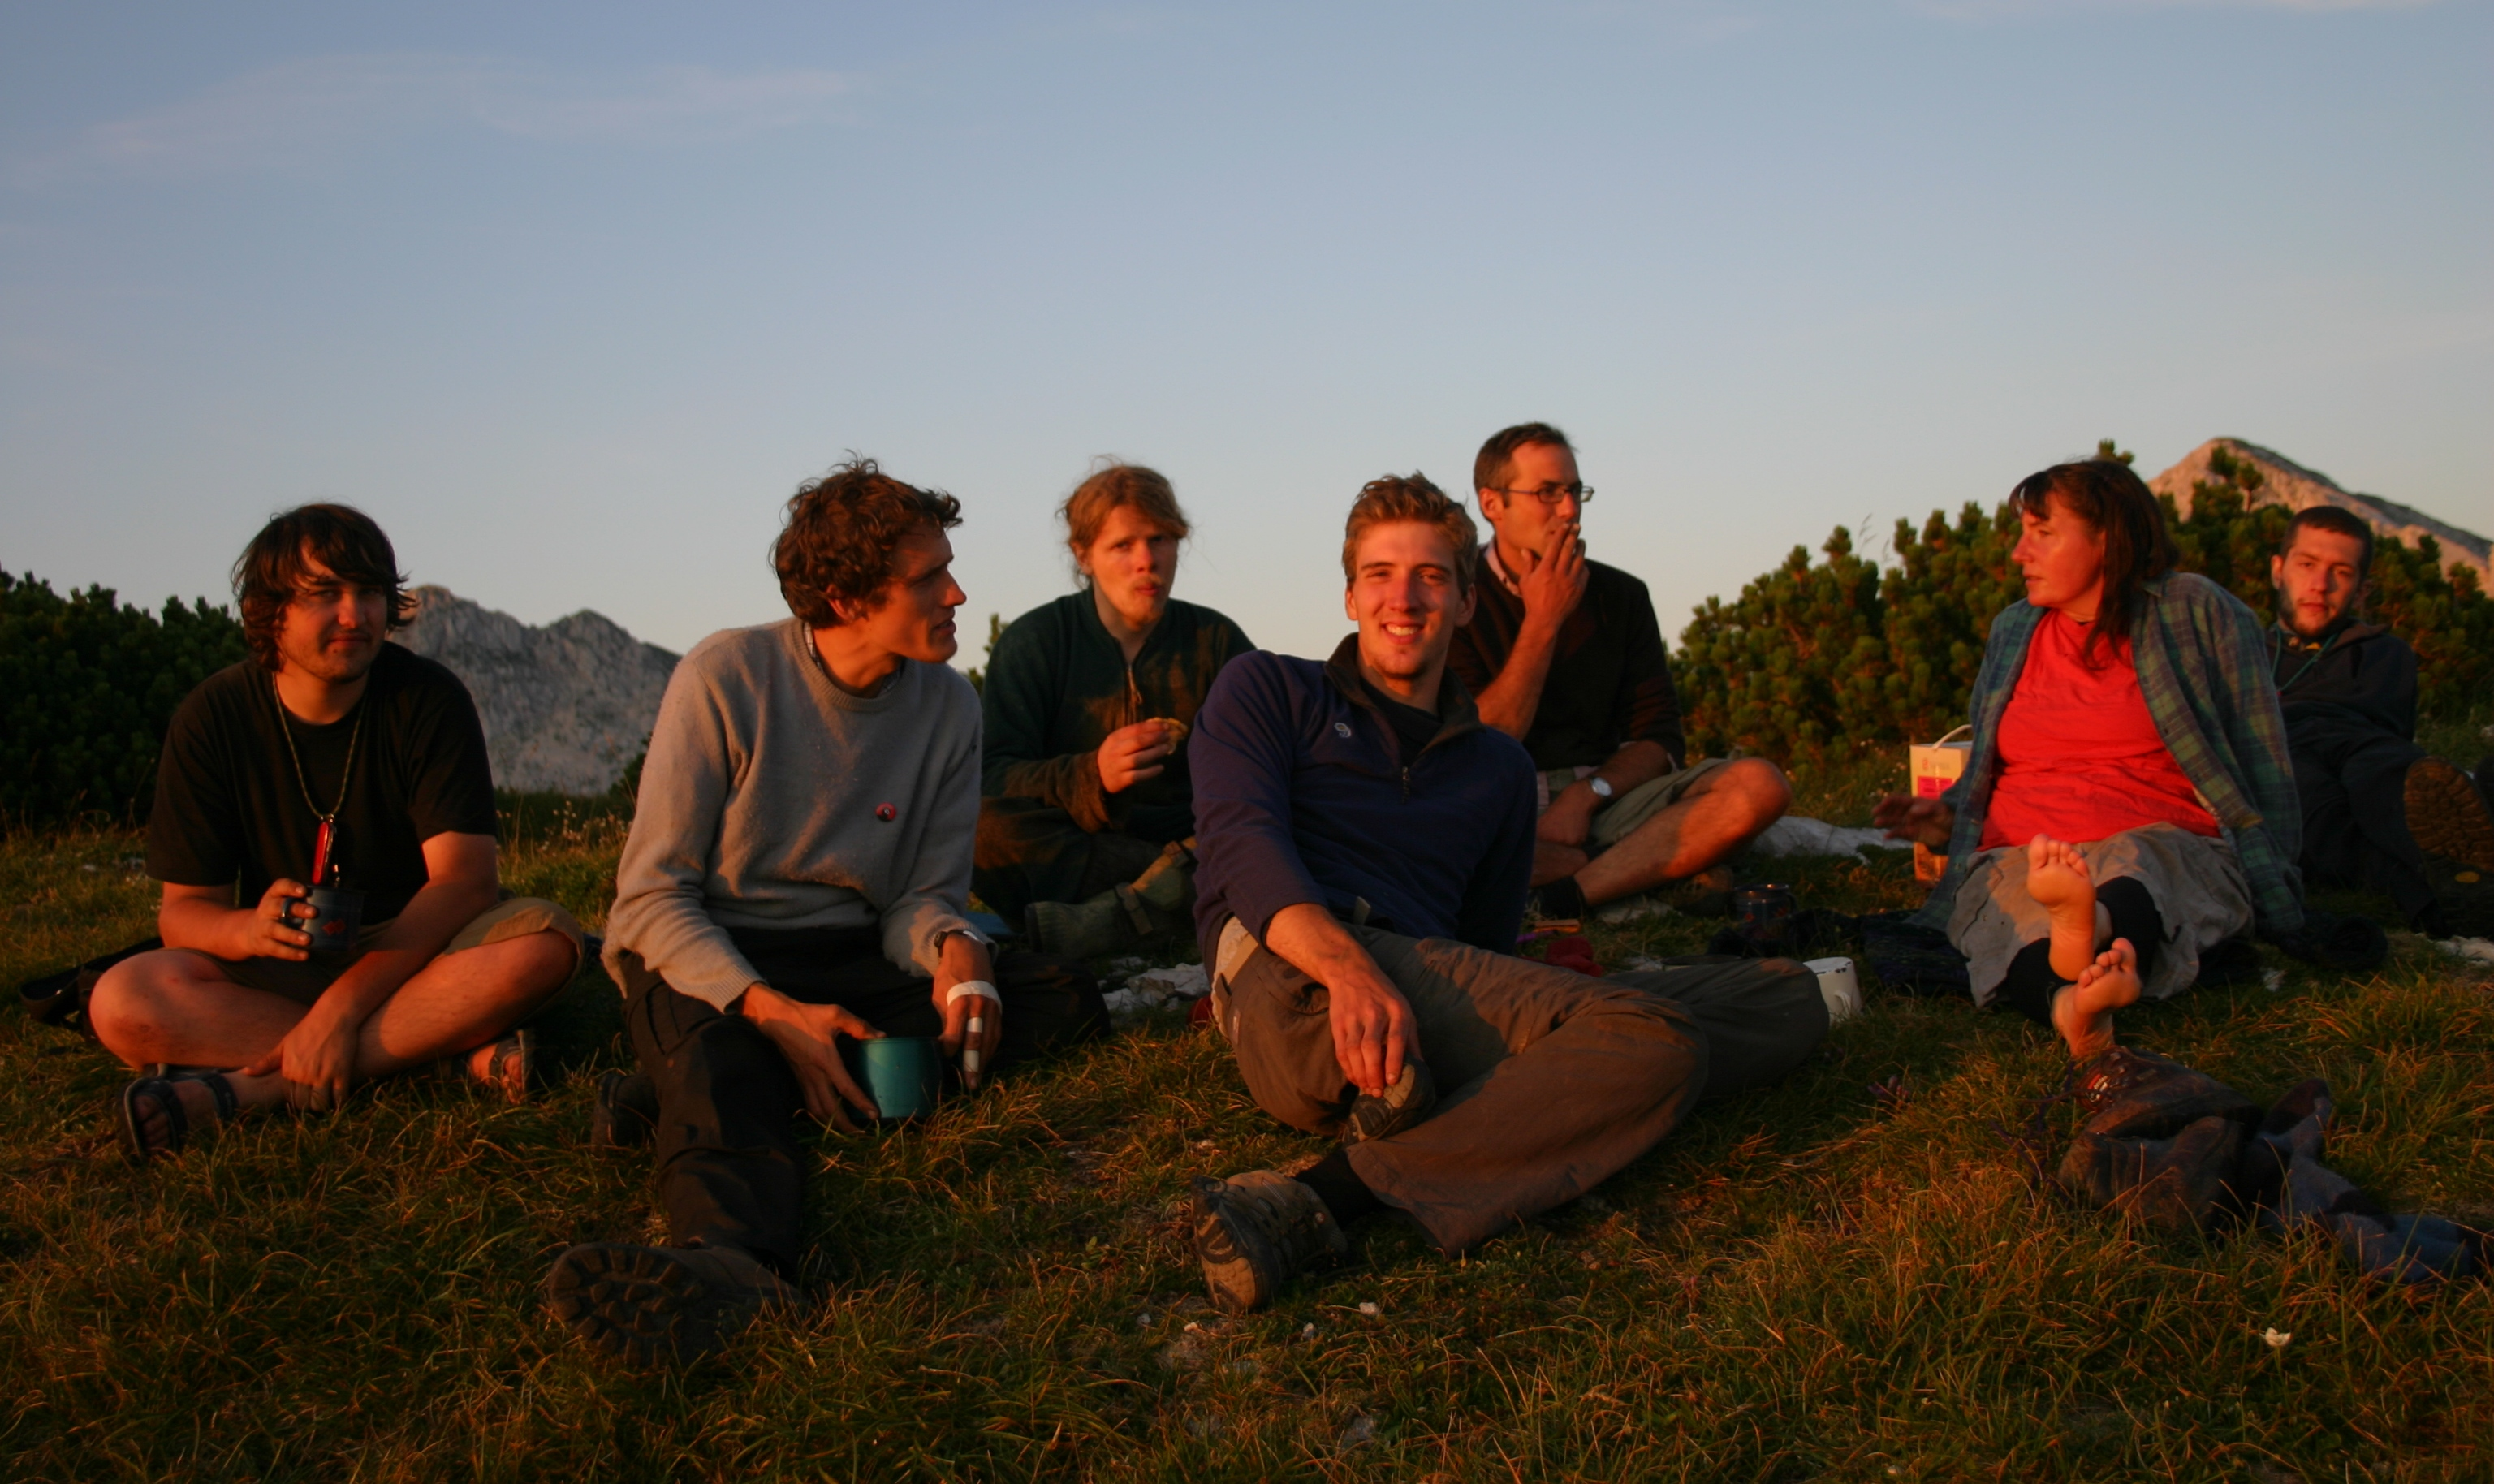
\includegraphics[width=\linewidth]{2009/achievements/2009-08-16-01.07.13 - Tharatorn Supasiti - Plateau at sunset 1 - IMG_5367--orig.jpg}}
\caption{\textit{left to right} Alex Herriott, Jarvist Frost, William French, Tim Osborne, James Hooper, Janet Cotter, Dan Greenwald. \pic{Tharatorn Supasiti}} \label{expo 2009}
\end{pagefigure}